\chapter{Results and Discussion}\label{sec:results}
\section{Quantitative Comparison}
We compare EfficientNet (no attention) against EfficientNet+CBAM on identical splits. Metrics include accuracy, macro/weighted F1, ROC\textendash AUC (macro OvR), and PR\textendash AUC (macro). Attention improves several classes, while Hypertension remains challenging due to limited single\textendash label prevalence. Class weighting or multi\textendash label learning may further improve H.

As shown in Figure~\ref{fig:train_curves}, both variants converge smoothly; the CBAM model trends to higher validation accuracy and lower loss. Figure~\ref{fig:auc_curves} summarizes ROC\textendash AUC and PR\textendash AUC trajectories, indicating consistent gains with attention. Per\textendash class ROC/PR curves in Figure~\ref{fig:perclass_curves} highlight stronger separability for several classes under CBAM.

\section{Confusion Matrices}
We include count\textendash based confusion matrices with full class names. Notable confusions often occur between AMD and Myopia, and Hypertension with other vascular signs.

Figure~\ref{fig:cms} visualizes the test\textendash set confusion matrices for both models.

\section{Curves}\label{sec:results_figs}
Training/validation curves (accuracy, loss, ROC\textendash AUC, PR\textendash AUC) and per\textendash class ROC/PR curves are provided to illustrate convergence behavior and separability across classes.

\begin{figure}[t]
  \centering
  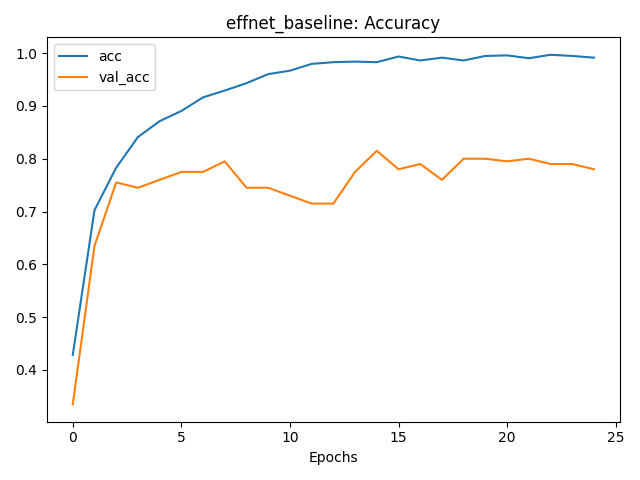
\includegraphics[width=0.48\textwidth]{effnet_baseline_acc.png}
  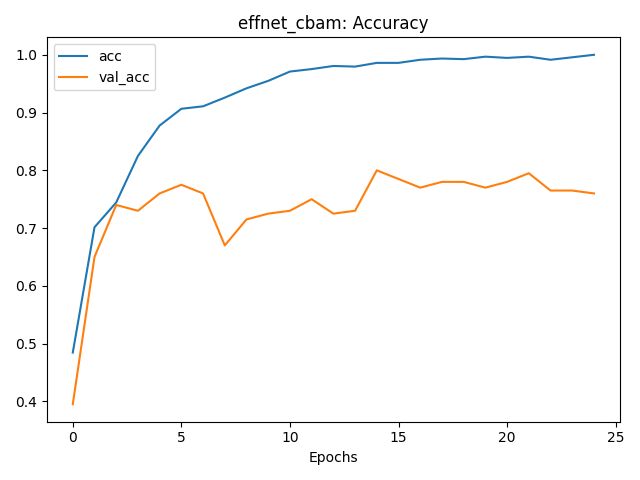
\includegraphics[width=0.48\textwidth]{effnet_cbam_acc.png}\\
  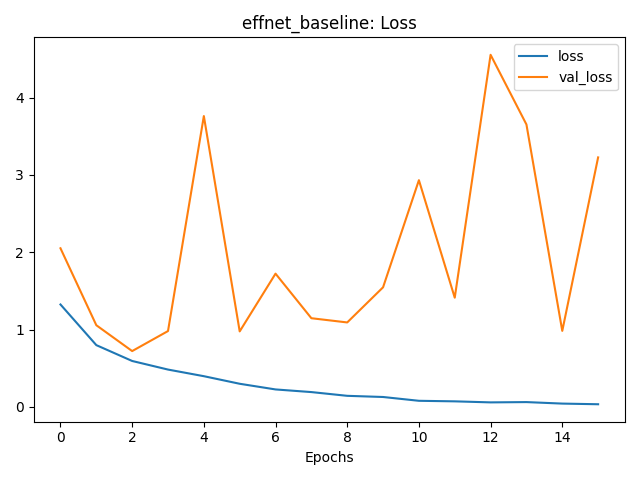
\includegraphics[width=0.48\textwidth]{effnet_baseline_loss.png}
  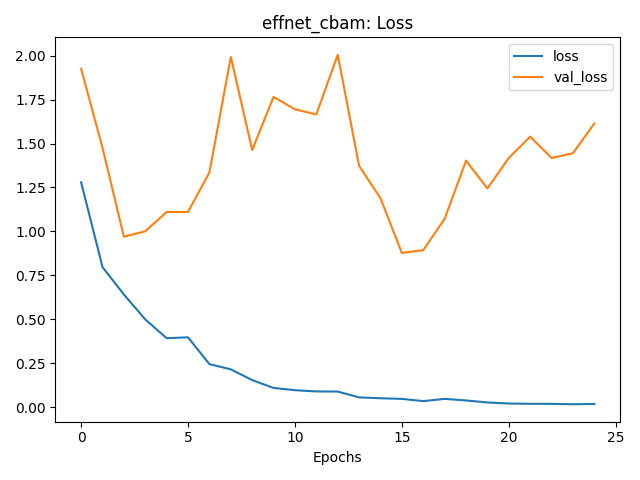
\includegraphics[width=0.48\textwidth]{effnet_cbam_loss.png}
  \caption{Training dynamics: accuracy (top) and loss (bottom) for EfficientNet baseline (left) and EfficientNet+CBAM (right).}
  \label{fig:train_curves}
\end{figure}

\begin{figure}[t]
  \centering
  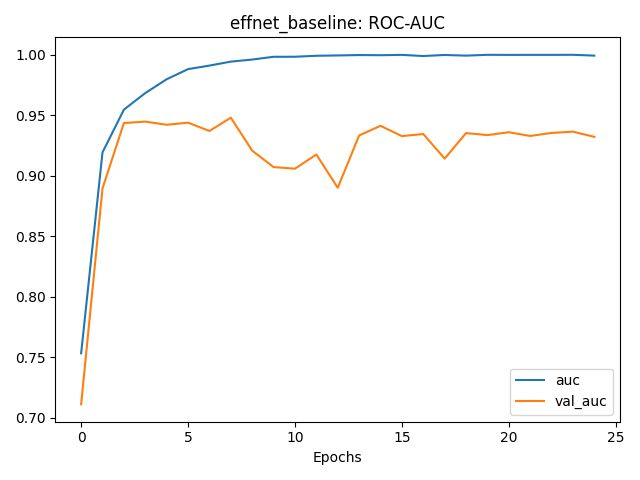
\includegraphics[width=0.48\textwidth]{effnet_baseline_auc.png}
  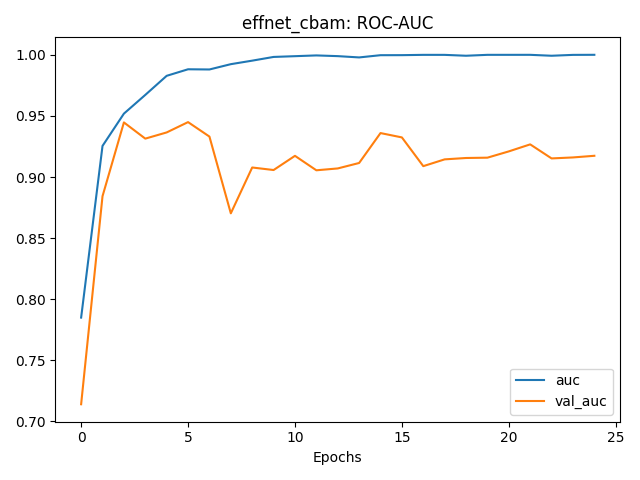
\includegraphics[width=0.48\textwidth]{effnet_cbam_auc.png}\\
  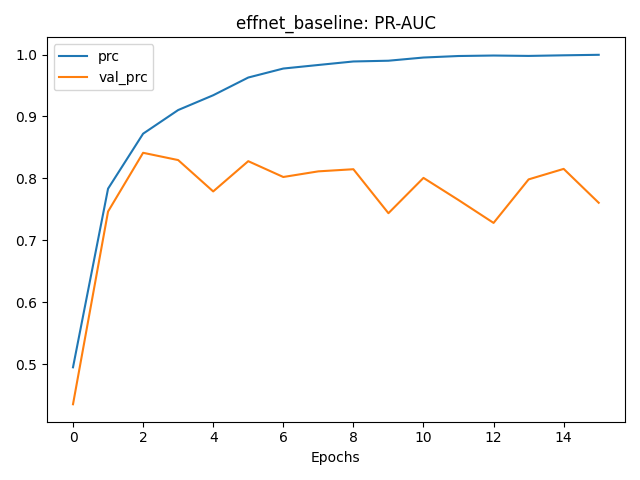
\includegraphics[width=0.48\textwidth]{effnet_baseline_prc.png}
  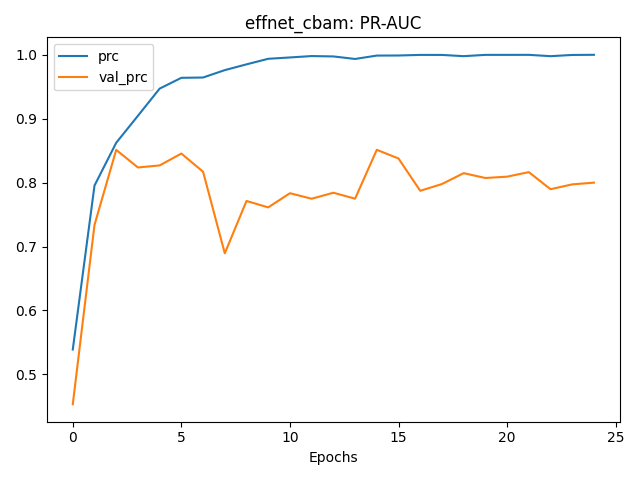
\includegraphics[width=0.48\textwidth]{effnet_cbam_prc.png}
  \caption{AUC metrics: ROC\textendash AUC (top) and PR\textendash AUC (bottom) for baseline (left) and CBAM (right).}
  \label{fig:auc_curves}
\end{figure}

\begin{figure}[t]
  \centering
  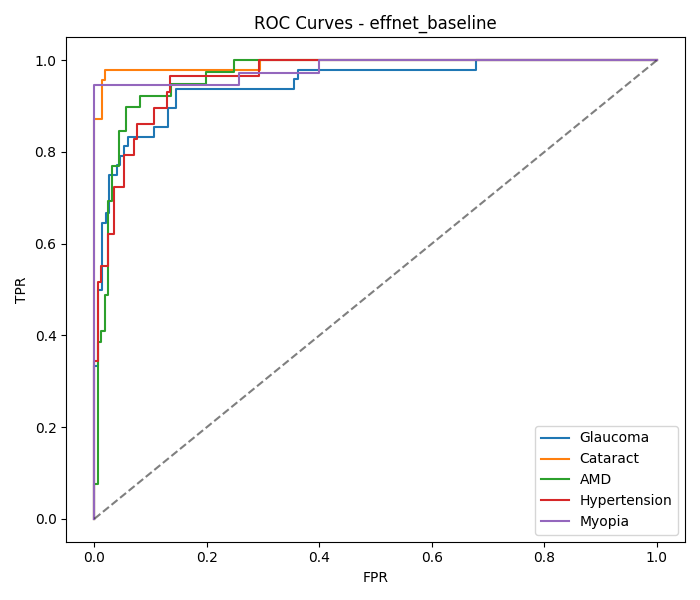
\includegraphics[width=0.48\textwidth]{roc_curves_effnet_baseline.png}
  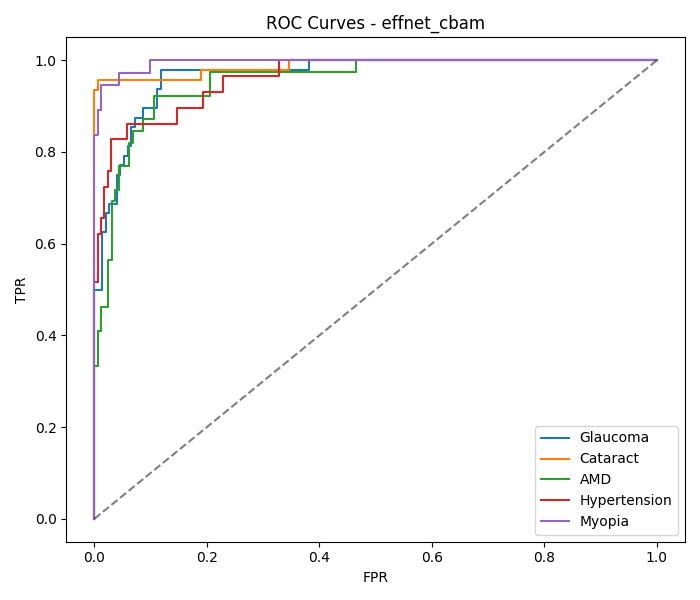
\includegraphics[width=0.48\textwidth]{roc_curves_effnet_cbam.png}\\
  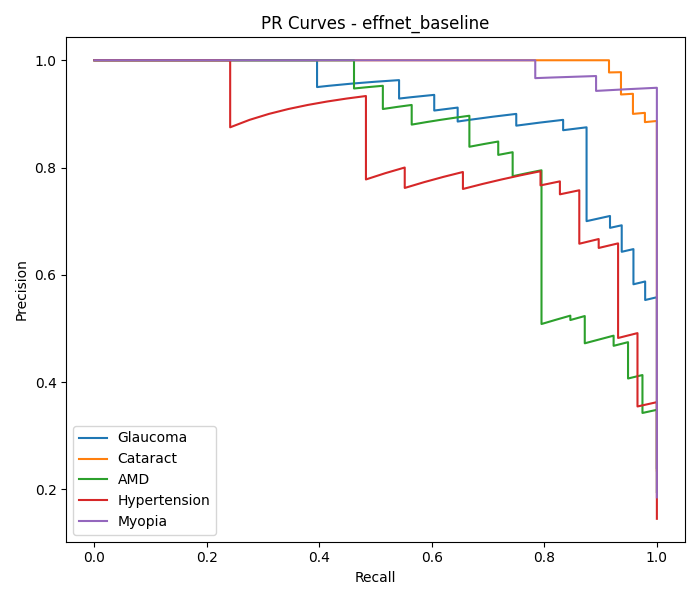
\includegraphics[width=0.48\textwidth]{pr_curves_effnet_baseline.png}
  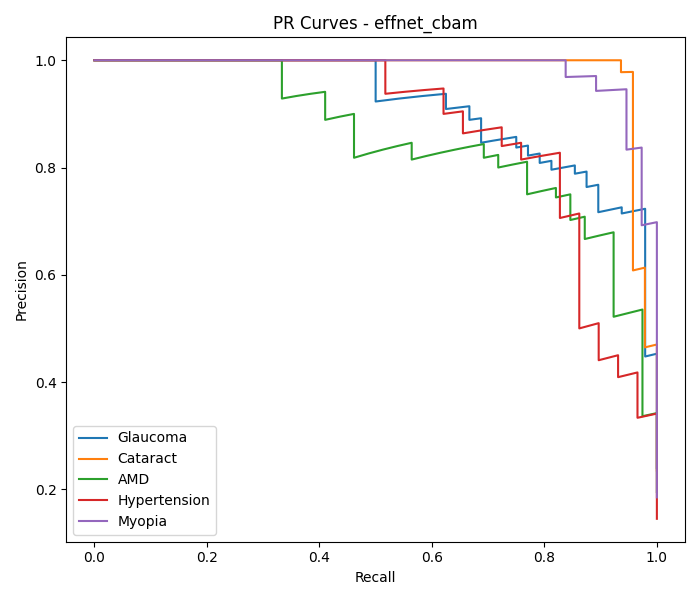
\includegraphics[width=0.48\textwidth]{pr_curves_effnet_cbam.png}
  \caption{Per\textendash class ROC (top) and PR (bottom) curves for baseline (left) vs. CBAM (right).}
  \label{fig:perclass_curves}
\end{figure}

\begin{figure}[t]
  \centering
  % Always use percent (row-normalized) confusion matrices (updated figures)
  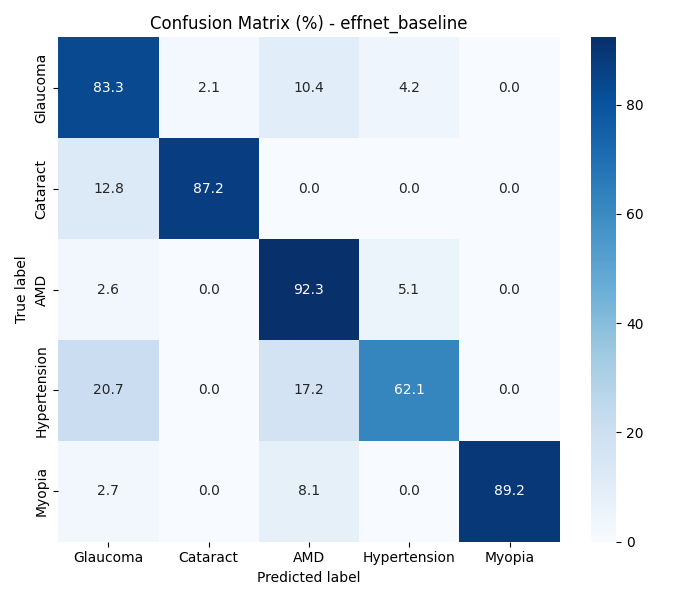
\includegraphics[width=0.48\textwidth]{cm_effnet_baseline_percent.png}
  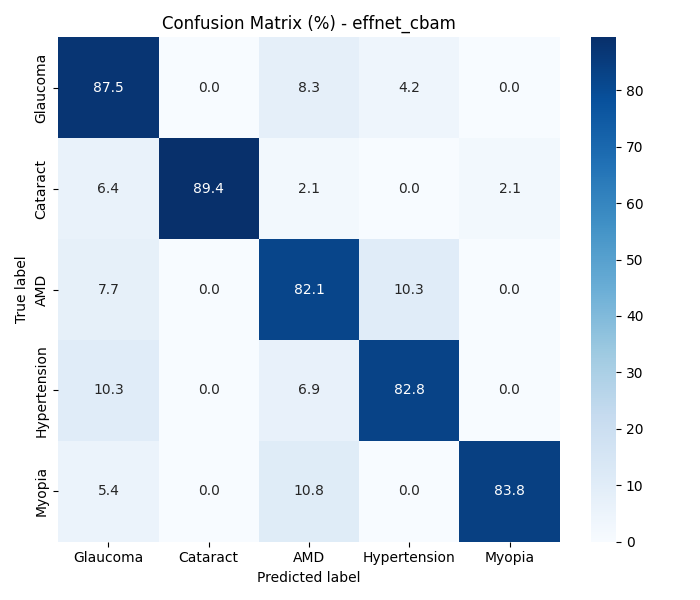
\includegraphics[width=0.48\textwidth]{cm_effnet_cbam_percent.png}
  \caption{Confusion matrices (row\textendash normalized percentages) on the held\textendash out test set for baseline (left) and CBAM (right).}
  \label{fig:cms}
\end{figure}

\section{Attention Visualization and Class Evidence}
To qualitatively benchmark attention, we show per\textendash class Grad\textendash CAM overlays comparing EfficientNet and EfficientNet+CBAM. Each panel annotates the model probability for the true class. We also include an eye\textendash image benchmarking section capturing representative samples for each class.

\begin{figure}[t]
  \centering
  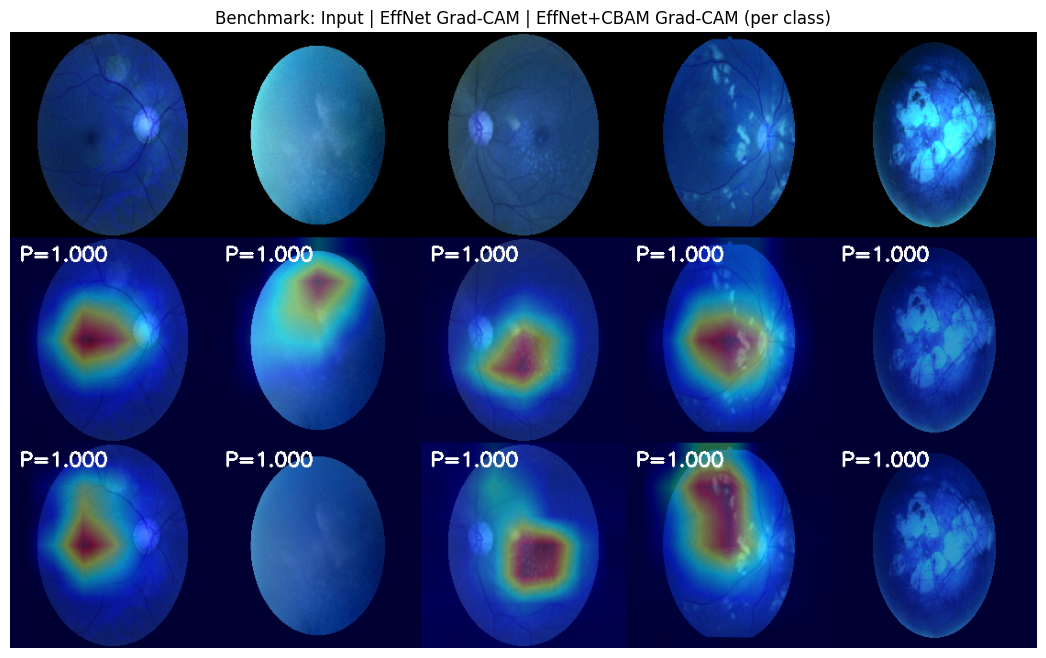
\includegraphics[width=0.98\textwidth]{../new_work/figures/gradcam_benchmark_panel.png}
  \caption{Per\textendash class benchmarking panel: for each class (left to right: Glaucoma, Cataract, AMD, Hypertension, Myopia), we show Input, EffNet Grad\textendash CAM, and EffNet+CBAM Grad\textendash CAM, with class probabilities.}
  \label{fig:gradcam_panel}
\end{figure}

\begin{figure}[t]
  \centering
  \setlength{\tabcolsep}{6pt}
  \begin{tabular}{ccccc}
    \textbf{G (Glaucoma)} & \textbf{C (Cataract)} & \textbf{A (AMD)} & \textbf{H (Hypertension)} & \textbf{M (Myopia)}\\
    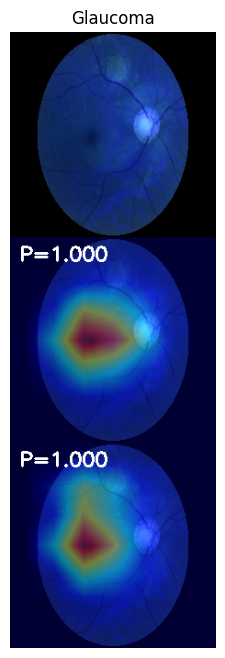
\includegraphics[width=0.18\textwidth]{../new_work/figures/gradcam_benchmark_Glaucoma.png} &
    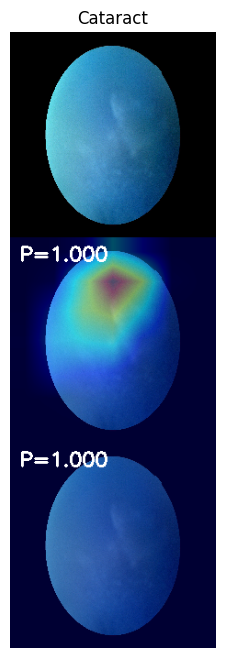
\includegraphics[width=0.18\textwidth]{../new_work/figures/gradcam_benchmark_Cataract.png} &
    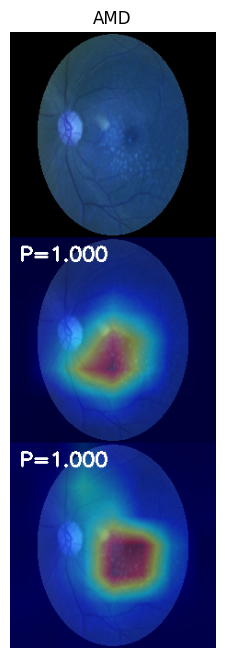
\includegraphics[width=0.18\textwidth]{../new_work/figures/gradcam_benchmark_AMD.png} &
    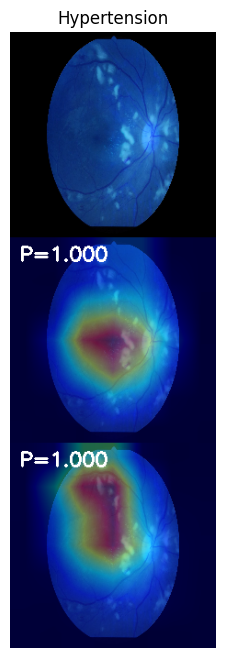
\includegraphics[width=0.18\textwidth]{../new_work/figures/gradcam_benchmark_Hypertension.png} &
    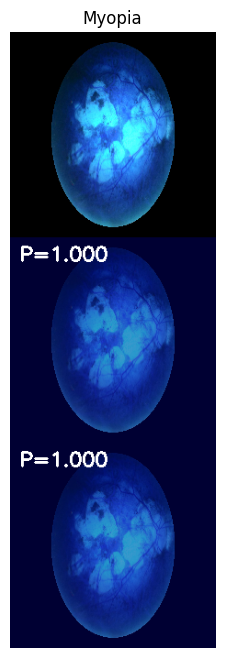
\includegraphics[width=0.18\textwidth]{../new_work/figures/gradcam_benchmark_Myopia.png} \\
  \end{tabular}
  \caption{Per\textendash class examples with explicit class names. Each column shows, from top to bottom: Input, EffNet Grad\textendash CAM (with P), and EffNet+CBAM Grad\textendash CAM (with P).}
  \label{fig:gradcam_perclass}
\end{figure}

\paragraph{Discussion.} Consistent with prior analyses of CBAM \cite{cbamDO,cbamMedium,woo2018cbam}, our overlays show that CBAM suppresses background and sharpens disease\textendash specific structures. For AMD and Myopia, CBAM concentrates on macular and optic\textendash disc vicinity more consistently than the baseline. Hypertension remains challenging due to scarce single\textendash label samples; however, row\textendash normalized confusion indicates improved precision compared to recall, suggesting additional class weighting and data curation can further benefit H.

